\documentclass{ximera}
\graphicspath{  %% When looking for images,
{./}            %% look here first,
{./pictures/}   %% then look for a pictures folder,
{../pictures/}  %% which may be a directory up.
{../../pictures/}  %% which may be a directory up.
{../../../pictures/}  %% which may be a directory up.
{../../../../pictures/}  %% which may be a directory up.
}

\usepackage{listings}
%\usepackage{circuitikz}
\usepackage{xcolor}
\usepackage{amsmath,amsthm}
\usepackage{subcaption}
\usepackage{graphicx}
\usepackage{tikz}
%\usepackage{tikz-3dplot}
\usepackage{amsfonts}
%\usepackage{mdframed} % For framing content
%\usepackage{tikz-cd}

  \renewcommand{\vector}[1]{\left\langle #1\right\rangle}
  \newcommand{\arrowvec}[1]{{\overset{\rightharpoonup}{#1}}}
  \newcommand{\ro}{\texttt{R}}%% row operation
  \newcommand{\dotp}{\bullet}%% dot product
  \renewcommand{\l}{\ell}
  \let\defaultAnswerFormat\answerFormatBoxed
  \usetikzlibrary{calc,bending}
  \tikzset{>=stealth}
  




%make a maroon color
\definecolor{maroon}{RGB}{128,0,0}
%make a dark blue color
\definecolor{darkblue}{RGB}{0,0,139}
%define the color fourier0 to be the maroon color
\definecolor{fourier0}{RGB}{128,0,0}
%define the color fourier1 to be the dark blue color
\definecolor{fourier1}{RGB}{0,0,139}
%define the color fourier 1t to be the light blue color
\definecolor{fourier1t}{RGB}{173,216,230}
%define the color fourier2 to be the dark green color
\definecolor{fourier2}{RGB}{0,100,0}
%define teh color fourier2t to be the light green color
\definecolor{fourier2t}{RGB}{144,238,144}
%define the color fourier3 to be the dark purple color
\definecolor{fourier3}{RGB}{128,0,128}
%define the color fourier3t to be the light purple color
\definecolor{fourier3t}{RGB}{221,160,221}
%define the color fourier0t to be the red color
\definecolor{fourier0t}{RGB}{255,0,0}
%define the color fourier4 to be the orange color
\definecolor{fourier4}{RGB}{255,165,0}
%define the color fourier4t to be the darker orange color
\definecolor{fourier4t}{RGB}{255,215,0}
%define the color fourier5 to be the yellow color
\definecolor{fourier5}{RGB}{255,255,0}
%define the color fourier5t to be the darker yellow color
\definecolor{fourier5t}{RGB}{255,255,100}
%define the color fourier6 to be the green color
\definecolor{fourier6}{RGB}{0,128,0}
%define the color fourier6t to be the darker green color
\definecolor{fourier6t}{RGB}{0,255,0}

%New commands for this doc for errors in copying
\newcommand{\eigenvar}{\lambda}
%\newcommand{\vect}[1]{\mathbf{#1}}
\renewcommand{\th}{^{\text{th}}}
\newcommand{\st}{^{\text{st}}}
\newcommand{\nd}{^{\text{nd}}}
\newcommand{\rd}{^{\text{rd}}}
\newcommand{\paren}[1]{\left(#1\right)}
\newcommand{\abs}[1]{\left|#1\right|}
\newcommand{\R}{\mathbb{R}}
\newcommand{\C}{\mathbb{C}}
\newcommand{\Hilb}{\mathbb{H}}
\newcommand{\qq}[1]{\text{#1}}
\newcommand{\Z}{\mathbb{Z}}
\newcommand{\N}{\mathbb{N}}
\newcommand{\q}[1]{\text{``#1''}}
%\newcommand{\mat}[1]{\begin{bmatrix}#1\end{bmatrix}}
\newcommand{\rref}{\text{reduced row echelon form}}
\newcommand{\ef}{\text{echelon form}}
\newcommand{\ohm}{\Omega}
\newcommand{\volt}{\text{V}}
\newcommand{\amp}{\text{A}}
\newcommand{\Seq}{\textbf{Seq}}
\newcommand{\Poly}{\textbf{P}}
\renewcommand{\quad}{\text{    }}
\newcommand{\roweq}{\simeq}
\newcommand{\rowop}{\simeq}
\newcommand{\rowswap}{\leftrightarrow}
\newcommand{\Mat}{\textbf{M}}
\newcommand{\Func}{\textbf{Func}}
\newcommand{\Hw}{\textbf{Hamming weight}}
\newcommand{\Hd}{\textbf{Hamming distance}}
\newcommand{\rank}{\text{rank}}
\newcommand{\longvect}[1]{\overrightarrow{#1}}
% Define the circled command
\newcommand{\circled}[1]{%
  \tikz[baseline=(char.base)]{
    \node[shape=circle,draw,inner sep=2pt,red,fill=red!20,text=black] (char) {#1};}%
}

% Define custom command \strikeh that just puts red text on the 2nd argument
\newcommand{\strikeh}[2]{\textcolor{red}{#2}}

% Define custom command \strikev that just puts red text on the 2nd argument
\newcommand{\strikev}[2]{\textcolor{red}{#2}}

%more new commands for this doc for errors in copying
\newcommand{\SI}{\text{SI}}
\newcommand{\kg}{\text{kg}}
\newcommand{\m}{\text{m}}
\newcommand{\s}{\text{s}}
\newcommand{\norm}[1]{\left\|#1\right\|}
\newcommand{\col}{\text{col}}
\newcommand{\sspan}{\text{span}}
\newcommand{\proj}{\text{proj}}
\newcommand{\set}[1]{\left\{#1\right\}}
\newcommand{\degC}{^\circ\text{C}}
\newcommand{\centroid}[1]{\overline{#1}}
\newcommand{\dotprod}{\boldsymbol{\cdot}}
%\newcommand{\coord}[1]{\begin{bmatrix}#1\end{bmatrix}}
\newcommand{\iprod}[1]{\langle #1 \rangle}
\newcommand{\adjoint}{^{*}}
\newcommand{\conjugate}[1]{\overline{#1}}
\newcommand{\eigenvarA}{\lambda}
\newcommand{\eigenvarB}{\mu}
\newcommand{\orth}{\perp}
\newcommand{\bigbracket}[1]{\left[#1\right]}
\newcommand{\textiff}{\text{ if and only if }}
\newcommand{\adj}{\text{adj}}
\newcommand{\ijth}{\emph{ij}^\text{th}}
\newcommand{\minor}[2]{M_{#2}}
\newcommand{\cofactor}{\text{C}}
\newcommand{\shift}{\textbf{shift}}
\newcommand{\startmat}[1]{
  \left[\begin{array}{#1}
}
\newcommand{\stopmat}{\end{array}\right]}
%a command to give a name to explorations and hints and theorems
\newcommand{\name}[1]{\begin{centering}\textbf{#1}\end{centering}}
\newcommand{\vect}[1]{\vec{#1}}
\newcommand{\dfn}[1]{\textbf{#1}}
\newcommand{\transpose}{\mathsf{T}}
\newcommand{\mtlb}[2][black]{\texttt{\textcolor{#1}{#2}}}
\newcommand{\RR}{\mathbb{R}} % Real numbers
\newcommand{\id}{\text{id}}
\newcommand{\coord}[1]{\langle#1\rangle}
\newcommand{\RREF}{\text{RREF}}
\newcommand{\Null}{\text{Null}}
\newcommand{\Nullity}{\text{Nullity}}
\newcommand{\Rank}{\text{Rank}}
\newcommand{\Col}{\text{Col}}
\newcommand{\Ef}{\text{EF}}
\newcommand{\boxprod}[3]{\abs{(#1\times#2)\cdot#3}}

\author{Zack Reed}
%borrowed from selinger linear algebra
\title{Finding Directions of Maximum Spread: SVD}
\begin{document}
\begin{abstract}

\end{abstract}
\maketitle


\section{Subspace Fitting and the SVD}

%\begin{outcome}
%  \begin{enumerate}
%  \item Compute the principal components of a matrix $A$.
%  \item Compute the centroid of a collection of data points.
%  \item Find the $k$-dimensional subspace that best approximates a
%    given collection of data points.
%  \item Find the $k$-dimensional affine subspace that best
%    approximates a given collection of data points.
%  \item Compute the total squared distance of the data points to the
%    best fit subspace (or best fit affine subspace).
%  \end{enumerate}
%\end{outcome}

In this section, we will more closely examine the geometric properties of the SVD that allow for analyses such as seen in \href{https://ximera.osu.edu/appliedlinearalgebra/c6ChapterSix/learningActivities/m6LearningActivities/leastSquares/leastSquaresApplicationVotingImages}{the Voting Records Application}.

Whereas in the previous section we considered the columns of a matrix from the standard transformational perspective, we now consider the $n$ columns of a matrix to be data points in $\RR^m$, where the matrix $A$ is $m\times n$. 


\begin{center}
  \begin{tikzpicture}[baseline=-0.5ex]
    \draw[thin,->] (-4,0) -- (4,0);
    \draw[thin,->] (0,-4) -- (0,4);
    % \draw[thick,blue] (-4,-4/1.29) -- (4,4/1.29);
    \fill[color=red] (-2.25,-1.21) circle (0.06);
    \fill[color=red] (-1.44,-1.28) circle (0.06);
    \fill[color=red] (2.29,1.82) circle (0.06);
    \fill[color=red] (0.25,0.43) circle (0.06);
    \fill[color=red] (-1.57,-1.07) circle (0.06);
    \fill[color=red] (2.51,2.00) circle (0.06);
    \fill[color=red] (-2.53,-2.34) circle (0.06);
    \fill[color=red] (-3.04,-2.40) circle (0.06);
    \fill[color=red] (0.84,0.36) circle (0.06);
    \fill[color=red] (-3.16,-2.73) circle (0.06);
    \fill[color=red] (-2.02,-1.88) circle (0.06);
    \fill[color=red] (3.06,2.44) circle (0.06);
    \fill[color=red] (-1.40,-1.12) circle (0.06);
    \fill[color=red] (-2.09,-1.34) circle (0.06);
    \fill[color=red] (-1.23,-1.13) circle (0.06);
    \fill[color=red] (0.48,0.06) circle (0.06);
    \fill[color=red] (-1.49,-1.20) circle (0.06);
    \fill[color=red] (0.98,0.75) circle (0.06);
    \fill[color=red] (1.40,0.89) circle (0.06);
    \fill[color=red] (-0.12,0.09) circle (0.06);
    \fill[color=red] (0.88,0.40) circle (0.06);
    \fill[color=red] (-0.38,0.55) circle (0.06);
    \fill[color=red] (0.34,0.46) circle (0.06);
    \fill[color=red] (0.45,0.21) circle (0.06);
    \fill[color=red] (-0.59,-0.63) circle (0.06);
    \fill[color=red] (-0.53,-0.29) circle (0.06);
    \fill[color=red] (2.10,1.35) circle (0.06);
    \fill[color=red] (1.65,1.60) circle (0.06);
    \fill[color=red] (-3.88,-2.83) circle (0.06);
    \fill[color=red] (-0.07,-0.01) circle (0.06);
    \fill[color=red] (-0.37,-0.57) circle (0.06);
    \fill[color=red] (-0.99,-0.75) circle (0.06);
    \fill[color=red] (-2.34,-2.08) circle (0.06);
    \fill[color=red] (3.63,3.15) circle (0.06);
    \fill[color=red] (1.37,0.48) circle (0.06);
    \fill[color=red] (-0.96,-0.74) circle (0.06);
    \fill[color=red] (3.51,2.79) circle (0.06);
    \fill[color=red] (-3.33,-2.72) circle (0.06);
    \fill[color=red] (0.39,0.09) circle (0.06);
    \fill[color=red] (-1.38,-1.17) circle (0.06);
    \fill[color=red] (-0.36,-0.65) circle (0.06);
    \fill[color=red] (1.38,0.66) circle (0.06);
    \fill[color=red] (1.85,1.24) circle (0.06);
    \fill[color=red] (2.35,1.85) circle (0.06);
    \fill[color=red] (0.85,0.25) circle (0.06);
    \fill[color=red] (-0.23,0.19) circle (0.06);
    \fill[color=red] (-0.90,-0.74) circle (0.06);
    \fill[color=red] (2.50,1.31) circle (0.06);
    \fill[color=red] (-0.45,-0.71) circle (0.06);
    \fill[color=red] (0.92,0.56) circle (0.06);
    \fill[color=red] (0.97,1.21) circle (0.06);
    \fill[color=red] (-0.85,-0.74) circle (0.06);
    \fill[color=red] (-0.10,0.13) circle (0.06);
    \fill[color=red] (0.32,0.49) circle (0.06);
    \fill[color=red] (2.58,1.57) circle (0.06);
    \fill[color=red] (-0.59,-0.48) circle (0.06);
    \fill[color=red] (2.28,1.50) circle (0.06);
    \fill[color=red] (1.21,0.94) circle (0.06);
    \fill[color=red] (-0.35,-0.13) circle (0.06);
    \fill[color=red] (-1.53,-1.26) circle (0.06);
    \fill[color=red] (-2.77,-2.14) circle (0.06);
    \fill[color=red] (1.23,1.02) circle (0.06);
    \fill[color=red] (2.61,1.88) circle (0.06);
    \fill[color=red] (-0.04,-0.05) circle (0.06);
    \fill[color=red] (2.09,1.30) circle (0.06);
    \fill[color=red] (2.37,1.52) circle (0.06);
    \fill[color=red] (-2.01,-1.69) circle (0.06);
    \fill[color=red] (0.48,0.72) circle (0.06);
    \fill[color=red] (0.23,0.49) circle (0.06);
    \fill[color=red] (-1.16,-0.95) circle (0.06);
    \fill[color=red] (-0.14,-0.18) circle (0.06);
    \fill[color=red] (-1.57,-1.68) circle (0.06);
    \fill[color=red] (0.39,0.15) circle (0.06);
    \fill[color=red] (-0.24,-0.29) circle (0.06);
  \end{tikzpicture}
\end{center}

You can manipulate and work with this data by loading $\texttt{+linalg/subspace\_fitting\_data.mat}$ in MATLAB.



Although these points are spread out in two dimensions, they seem to
be located pretty close to a 1-dimensional subspace. Probably the best
way to interpret this particular data set is to think of the points as
being ``essentially'' on a line, up to some small random errors. Note that this is the same principle we applied in the case of the voting application.

More generally, suppose we are given a collection of data points in
$n$-dimensional space, and we are looking for a $k$-dimensional
subspace that all data points are close to.  This is an important way
to make sense of high-dimensional data. For example, it would be very
difficult to visualize data in a $100$-dimensional space. However, it
we knew that the data points lie very close to a 2-dimensional
subspace, then we could project all of the points to the subspace to
obtain a 2-dimensional image of the data.

To state the problem more precisely, let us introduce the following
notation. If $W$ is a subspace of $\R^n$ and $\vect{v}\in\R^n$ is a
vector, let us write $d(\vect{v},W)$ for the shortest distance from
$\vect{v}$ to $W$ (i.e., the distance from $\vect{v}$ to $W$ along a
line that is perpendicular to $W$). Moreover, if $W$ is a subspace of
$\R^n$ and $\vect{v}_1,\ldots,\vect{v}_m\in\R^n$ are the position
vectors of $m$ points, we define the \textbf{total squared distance}%
\index{distance!total squared distance}%
\index{squared distance}%
\index{total squared distance}%
\index{subspace fitting!total squared distance} of the points to
the subspace to be the quantity
\begin{equation*}
  D = d(\vect{v}_1,W)^2 + \ldots + d(\vect{v}_m,W)^2.
\end{equation*}

You can visualize this phenomenon in $2$-dimensions with the following GeoGebra application:

\begin{center}
  \geogebra{tfds5q4w}{552}{576}
\end{center}



You can enter and alter points in Vector Lists 1 and 2 to change the data points you want to visualize with green dots. A line through the origin is visualzied in blue, and can be rotated by clicking and dragging the blue dot at the end of the direction vector $\vec{v}$. If you keep ``Emphasize Distances to Line" checked, you will see the distances $d(\vec{v}_i,L)$ from the points to the line visualized, and will also see a calculation ``Distance Square Sum='' which automatically calculates the sum of square distances \begin{equation*}
  D = d(\vect{v}_1,L)^2 + \ldots + d(\vect{v}_m,L)^2
\end{equation*} for you.

The goal of describing high-dimensional data using low-dimensional subspaces that ``closely approximate'' the data is akin to finding subspaces that minimize the sum of square distances from the data to the subspace, and can be generally stated as follows:


 
\begin{problem}\name{Subspace fitting problem}\label{prop:subspace-fitting}

  Given vectors $\vect{v}_1,\ldots,\vect{v}_m\in\R^n$ and given an
  integer $k\leq n$, find the $k$-dimensional subspace
  $W\subseteq\R^n$ that minimizes the total squared distance, i.e.,
  such that $D$ is as small as possible%
  \index{subspace fitting}%
  \index{fitting!subspace fitting}.
\end{problem}

\begin{example}{Subspace fitting in $\R^2$}{subspace-fitting-r2}
  Consider the following collection of points in $\R^2$:
  \begin{equation*}
    \set{
      \startmat{r}  2 \\ -3 \stopmat,
      \startmat{r} -1 \\  0 \stopmat,
      \startmat{r}  2 \\  3 \stopmat,
      \startmat{r} -6 \\ -7 \stopmat,
      \startmat{r}  6 \\ 11 \stopmat,
      \startmat{r}  0 \\ -1 \stopmat,
      \startmat{r}  1 \\  6 \stopmat,
      \startmat{r} -2 \\ -3 \stopmat,
      \startmat{r} -7 \\ -6 \stopmat
    }.
  \end{equation*}
  Find the 1-dimensional subspace that best approximates this
  collection of points. What is the total squared distance of the
  points to the subspace?
\end{example}


  The space $W$ is shown in the following illustration, along with the
  original points:
  \begin{center}
    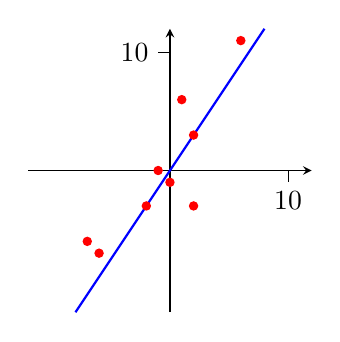
\begin{tikzpicture}[scale=0.15]
      \draw[thin,->] (-12,0) -- (12,0);
      \draw[thin,->] (0,-12) -- (0,12);
      \draw[thin] (0,10) -- (-1,10) node[left] {$10$};
      \draw[thin] (10,0) -- (10,-1) node[below] {$10$};
      \draw[thick,blue] (-8,-12) -- (8,12);
      \fill[color=red] (2,-3) circle (0.4);
      \fill[color=red] (-1, 0) circle (0.4);
      \fill[color=red] (2, 3) circle (0.4);
      \fill[color=red] (-6, -7) circle (0.4);
      \fill[color=red] (6, 11) circle (0.4);
      \fill[color=red] (0, -1) circle (0.4);
      \fill[color=red] (1, 6) circle (0.4);
      \fill[color=red] (-2, -3) circle (0.4);
      \fill[color=red] (-7, -6) circle (0.4);
    \end{tikzpicture}
  \end{center}
  Of course, in real life the data is much more complex than in this example




\begin{example}\name{Subspace fitting in $\R^3$}\label{ex:subspace-fitting-r3}
  Consider the following collection of points in $\R^3$:
  \begin{equation*}
    \set{
      \startmat{r} -7 \\ 4 \\ 5 \stopmat,
      \startmat{r} 0 \\ 3 \\ 3 \stopmat,
      \startmat{r} 2 \\ -5 \\ -4 \stopmat,
      \startmat{r} 10 \\ -4 \\ 1 \stopmat,
      \startmat{r} -2 \\ 5 \\ 4 \stopmat,
      \startmat{r} -8 \\ -1 \\ -5 \stopmat,
      \startmat{r} 5 \\ 4 \\ 2 \stopmat,
      \startmat{r} -6 \\ 9 \\ 6 \stopmat,
      \startmat{r} 9 \\ -6 \\ 3 \stopmat,
      \startmat{r} -2 \\ -7 \\ -8 \stopmat
    }.
  \end{equation*}
  %\begin{enumialphparenastyle}
    \begin{enumerate}
    \item Find the 1-dimensional subspace that best approximates this
      collection of points.
    \item Find the 2-dimensional subspace that best approximates this
      collection of points.
    \item What is the 3-dimensional subspace that best approximates this
      collection of points?
    \end{enumerate}
  %\end{enumialphparenastyle}
  In each case, what is the total squared distance of the points to
  the subspace?
\end{example}



\section*{Maximizing Spread, Minimizing Distance, Computing the SVD}

We now hone in on how the way that the SVD is constructed, which brings together a few key ideas including why the SVD gives us the best-fitting (in the sense of distance minimization) subspaces. 

The key is the interplay between \emph{minimizing square distances} and \emph{maximizing projection spread}. These are crucially linked together, which allows us to leverage an algorithm that finds direction of maximum projection spread to construct the SVD. 

\subsection*{Maximizing Spread and Minimizing Square Distances}

Let's return to the GeoGebra applet, but ask more targeted questions. First, consider the applet with just the first vector in list 1, $\begin{bmatrix}
  1\\.5
\end{bmatrix}$ (set Vector List 2 to just the zero vector).

\begin{center}
  \geogebra{tfds5q4w}{552}{576}
\end{center}

As you rotate the unit direction vector $\vec{v}$, if you select ``Emphasize Distances to Line", the applet will show the orthogonal projection of the data point to the line. If you select ``Emphasize Projection Vectors", the applet will de-emphasize the distance to the line and instead emphasize the length of the projection vector along the line. 

Which of the following statements is true of the relationship between the distances to and projections along the possible lines?



\begin{problem}

  \begin{selectAll}
  
    \choice{The $\vec{v}$ whose line minimizes the data distance is orthogonal to the vector $\vec{w}$ that maximizes the projection length of the data.}
    \choice{There is only one $\vec{v}$ that minimizes the distance of the data to the line.}
    \choice[correct]{The $\vec{v}$ whose line minimizes the data distance is parallel to the vector $\vec{w}$ that maximizes the projection length of the data.}

  \end{selectAll}

  \begin{feedback}
  
    With one data point, the distance-minimizing line crosses through the data point itself, and there are two vectors that acheive this (or rather, one vector and its negative). In this case $\pm \begin{bmatrix}
      .893\\.45
    \end{bmatrix}$. All other directions increase the distance from the data to the line. If you switch to ``Emphasize Projeciton Vectors'', you'll note that the length of the projection vector equals $1.25$ when the data point is on the line, and then only decreases when the data point is off of the line, being zero when the projection distance vector is orthogonal to the line. 

    As such, the line that minimizes the projection distance is also the line that maximizes the length of the projection vector.

    In fact, this is due to the Pythagorean Theorem. The norm of the data point vector is fixed, and so the data point vector, the distance to the projection, and the length of the projection make a right triangle.

    \begin{center}
      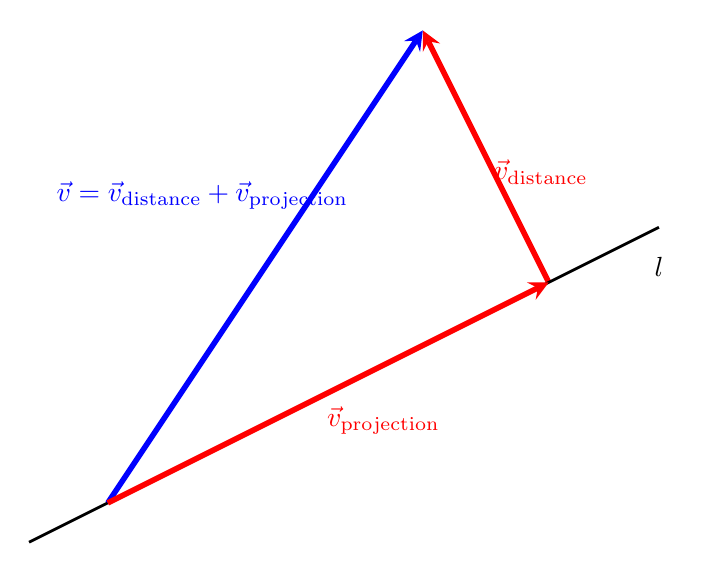
\begin{tikzpicture}
       \draw[line width=2pt,red,-stealth](3.6, 0.8)--(2,4);
       \node[red] at (3.5, 2.2)   (a) {$\vec{v}_{\text{distance}}$};
      \node[red] at (1.5, -0.95)   (b) {$\vec{v}_{\text{projection}}$};
       \node[] at (5, 1)   (c) {$l$};
       \node[blue] at (-0.8, 1.9)   (d) {$\vec{v}=\vec{v}_{\text{distance}}+\vec{v}_{\text{projection}}$};
        \draw [-,line width=1pt]  (-3,-2.5)--(5, 1.5);
     \draw[line width=2pt,blue,-stealth](-2, -2)--(2,4);
     \draw[line width=2pt,red,-stealth](-2, -2)--(3.6, 0.8);
     \end{tikzpicture}
       
     \end{center}

     Because the projection is orthogonal, we always have this right triangle, so 

     $$\left\|\vec{v}\right\|=\left\|\vec{v}_{\text{distance}}\right\|+\left\|\vec{v}_{\text{projection}}\right\|,$$

     meaning increasing the proejction or distance length will necessarily decrease the other.

  \end{feedback}



\end{problem}



In fact, this dynamic between the projection lengths and the projection distances is true for any number of data points, not just one data point, since each data point makes a right triangle via orthogonal projection along any line (unless the point lies on the line).

So, if \begin{equation*}
  D = d(\vect{v}_1,W)^2 + \ldots + d(\vect{v}_m,W)^2
\end{equation*} represents the sum of square projection distances, then we use the shorthand $p(\vect{v},W)^2$ for the square projection length of a vector onto a subspace and can say that the sum of square projection lengths \begin{equation*}
  P = p(\vect{v}_1,W)^2 + \ldots + p(\vect{v}_m,W)^2
\end{equation*} increases as $D$ decreases and vice versa. We'll call $P$ the \emph{spread} of the data along the subspace $W$.

More pointedly, we can turn this into a useful theorem for finding the SVD.

\begin{theorem}\name{Maximizing Spread and Minimizing Distance}
  If $A$ is an $m\times n$ matrix, then a subspace $W$ of $\RR^m$ that maximizes the spread of the columns of $A$ also minimizes the distances of the columns of $A$ to $W$ in $\RR^m$.
\end{theorem}

$P$ actually relates very closely to an important norm on {\bf matrices}, called the \emph{Frobenius Norm}.

\begin{definition}
  Let $A$ be an $m\times n$ matrix with columns denoted $a_i$. Then $\sqrt{P}$ is the Frobenius Norm of $A$, denoted $\left\|A\right\|_F$. 

  In other words, $\left\|A\right\|_F=\sqrt{\sum_{i=1}^n\left\|a_i\right\|}$.
\end{definition}

\subsection*{An algorithm for computing the SVD}

This brings us to one way to compute the SVD! We will not be doing this ourselves explicitly, but it is always important to know how useful tools such as the SVD are built so that we can understand why they work the way they do. 

There are four important features of singular values and singular vectors that contribute to their construction: \begin{enumerate}
  \item The singular vectors represent the directions of maximum projection spread, $P$,
  \item The singular values quantify that spread, and 
  \item The singular vectors form orthonormal bases of $\RR^m$ and $\RR^n$
  \item The SVD factors $A$ into $U*S*V^T$.
\end{enumerate}

With these features in mind, the SVD production algorithm is as follows.

\begin{theorem}{SVD-Producing Algorithm}

  Given a $m\times n$ matrix $A$, one can find the SVD of $A$ by taking the following steps:

  \begin{enumerate}
    \item Find a direction vector $\vec{v}_1$ that maximizes $\left\|A\vec{v}\right\|$ over all unit vectors $\vec{v}$. $\vec{v}_1$ is the first right singular vector, and call $\sigma_1=\left\|A\vec{v}_1\right\|$ the first singular value. 
    \item Find the second right singular vector $\vec{v}_2$ by maximizing $\left\|A\vec{v}\right\|$ over all unit vectors $\vec{v}$ that are orthogonal to $\vec{v}_1$. The second singular value is $\sigma_2=\left\|A\vec{v}_2\right\|$. 
    \item Repeat until you have found a sufficient number of right singular vectors and singular values.
    \item Form the left singular vectors from the matrix products $\vec{u}_i=\frac{A\vec{v}_i}{\sigma_i}$.
  \end{enumerate}

  There are other ways to compute the SVD more efficiently and with connections to other concepts to be explored in future modules, but this first cosntruction method emphasizes that the singular vectors are built to maximize the spread of the vectors along the projected subspaces, that the singular values quantify the spread along the projected subpsaces, and that the singular vectors form orthonormal bases of $\RR^m$ and $\RR^n$. 

  Indeed, because matrix multiplication gives the dot product of each row $A$ with the vector $\vec{v}$, $\left\|A\vec{v}\right\|^2$ is the same computation as $P$, the spread of the vectors along the projection in the direction of $\vec{v}$. Hence, maximizing $\left\|A\vec{v}\right\|$ also maximizes $\left\|A\vec{v}\right\|^2=P$. As we've already discussed, maximizing $P$ is the same as minimizing $D$, so we have found the sequence of basis vectors from which to construt best-fitting subspaces.

  For a more detailed analysis of this process, see Blum, Hopcroft, and Kannan's \emph{Foundations of Data Science} (2015). A free pdf version can be found \href{https://www.cs.cornell.edu/jeh/book.pdf}{here}.

\end{theorem}

\end{document}